% !TEX TS-program = pdflatex
% !TEX encoding = UTF-8 Unicode
% !TEX root = ../main.tex
% !TEX spellcheck = en-US
% ****************************************************************************************
% File: purpose_and_scope.tex
% Author: Patrick Haselwanter
% Date: 2023-10-28
% ****************************************************************************************
\chapter{Usage}
\label{chapter:additional_functionalities}

The \texttt{turtlesimAutomata} package can be used in combination with the \texttt{turtlesim\_teleop} package, which allows the user to manually control the turtle in the turtlesim environment, whilst still mainting the automatic behaviour provided by the \texttt{turtlesimAutomata} package. This may result in interesting behaviour, as shown in \autoref{fig:example_teleop}.

\begin{figure}[htbp]
    \centering
    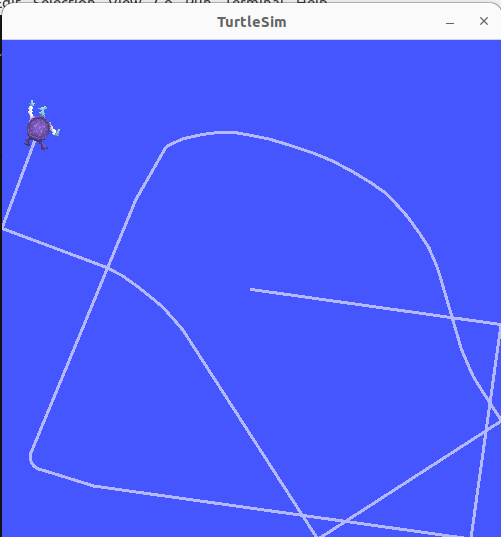
\includegraphics[width=0.5\textwidth]{./img/turtle_teleop_example.png}
    \caption{\texttt{turtlesimAutomata} and \texttt{turtlesim\_teleop} working together}
    \label{fig:example_teleop}
\end{figure}

\autoref{fig:rqt_graph_teleop} shows the \texttt{rqt\_graph} of the \texttt{turtlesimAutomata} and \texttt{turtlesim\_teleop} packages working together.

\begin{figure}[htbp]
    \centering
    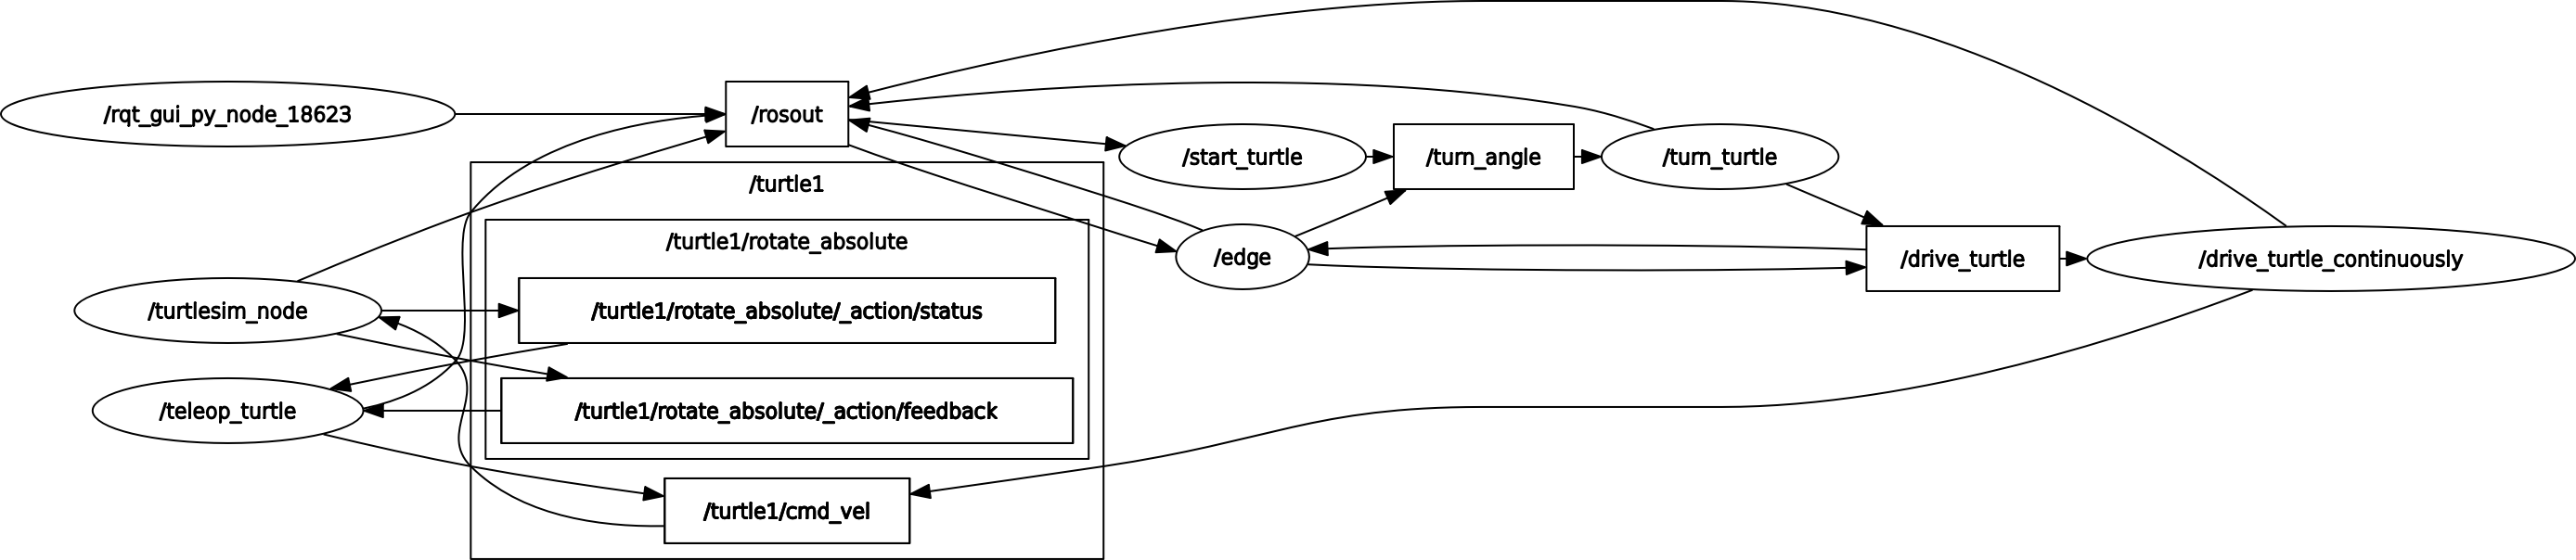
\includegraphics[width=1\textwidth]{./img/rosgraph_teleop.png}
    \caption{turtlesimAutomata and \texttt{turtlesim\_teleop} working together shown in \texttt{rqt\_graph}}
    \label{fig:rqt_graph_teleop}
\end{figure}

% EOF